\chapter{\label{intro}Introduction}

High energy physics is about understanding elementary particles that are fundamental constituents of matter.  Experimental high-energy physics (HEP) focuses on two primary goals that are interconnected, which seek novel particles associated with physics beyond the Standard Model(BSM) and Standard Model(SM) particles with high precision\cite{Salam:1964ry}\cite{GLASHOW1961579}. The standard model had correctly predicted the existence of $W^\pm$ and Z bosons along with the top quark\cite{PhysRevLett.19.1264}\cite{10.1143/PTP.49.634}. The Higgs boson discovery in 2012 at the LHC(CERN) further upholds the model\cite{Aad_2015}.

\autoref{fig:my_figure_1} lists standard model particles with the known three generations of leptons and quarks, the gauge bosons, and Higgs boson. The leptons and quarks make up matter, whereas the gauge bosons mediate the interactions among them\cite{PhysRevLett.13.321}. All massive fundamental particles in the Standard Model get their masses through the Brout-Englert-Higgs (BEH) mechanism\cite{Higgs:1964pj}.

For SM and BSM, rare signals need to be identified from vast backgrounds. This becomes an important issue as the number of pile-up collisions with additional protons in the bundle at  HL-LHC increases significantly\cite{https://doi.org/10.48550/arxiv.1807.02876}. This have been helped by the introduction of machine learning techniques. Machine learning algorithms are state-of-the-art in event and particle identification, energy estimation, and pile-up suppression applications in HEP. By using machine learning techniques to study the laws governing the structure of matter and  its interactions\cite{Baldi2014}.

Observing and studying these particles can reveal crucial information on the nature of matter\cite{Higgs_snowmass}. Such discoveries necessitate the use of sophisticated statistical approaches, and the use of machine learning tools. Improvements in analytical techniques immediately raise particle discovery potential, given the limited quantity and high cost of data.



% Chapter 1: Introduction
%     \begin{itemize}
%         \item SM
%         \item BSM
%         \item VLQ
%         \item Signal and Background Topology 
%         \item CMS
%         \item Objective of your experiment
%             \end{itemize}
    
% chapter 2: Machine Learning
% Chapter 3:  Simulated Samples
% \begin{itemize}
%     \item About CMS
%     \item about how can it be helpful for your work
%     \item how data are simualtad 
%     \item how you obtained the data
%     \item as written in the last report

% \end{itemize}

% Chapter 4:Analysis Strategies\\

% chapter 5:- Results and Discussion\\
% ch-6: summary and Conclusion



\section{Standard Model and shortcomings}

The Standard Model of particle physics(\autoref{fig:my_figure_1})is a model attempt to explain events and phenomena in the universe. The Standard Model(SM) of fundamental interaction, which has been successfully tested for the past 30 years, confirms its dynamics in the gauge sector and flavour structure, including a compelling confirmation of the reason of observable parity violations(P) and coupled charge and parity symmetry(CP). However, this is an incomplete theory and does not explain many  observed or unobserved events, such as:
\begin{figure}[H]
    \centering
    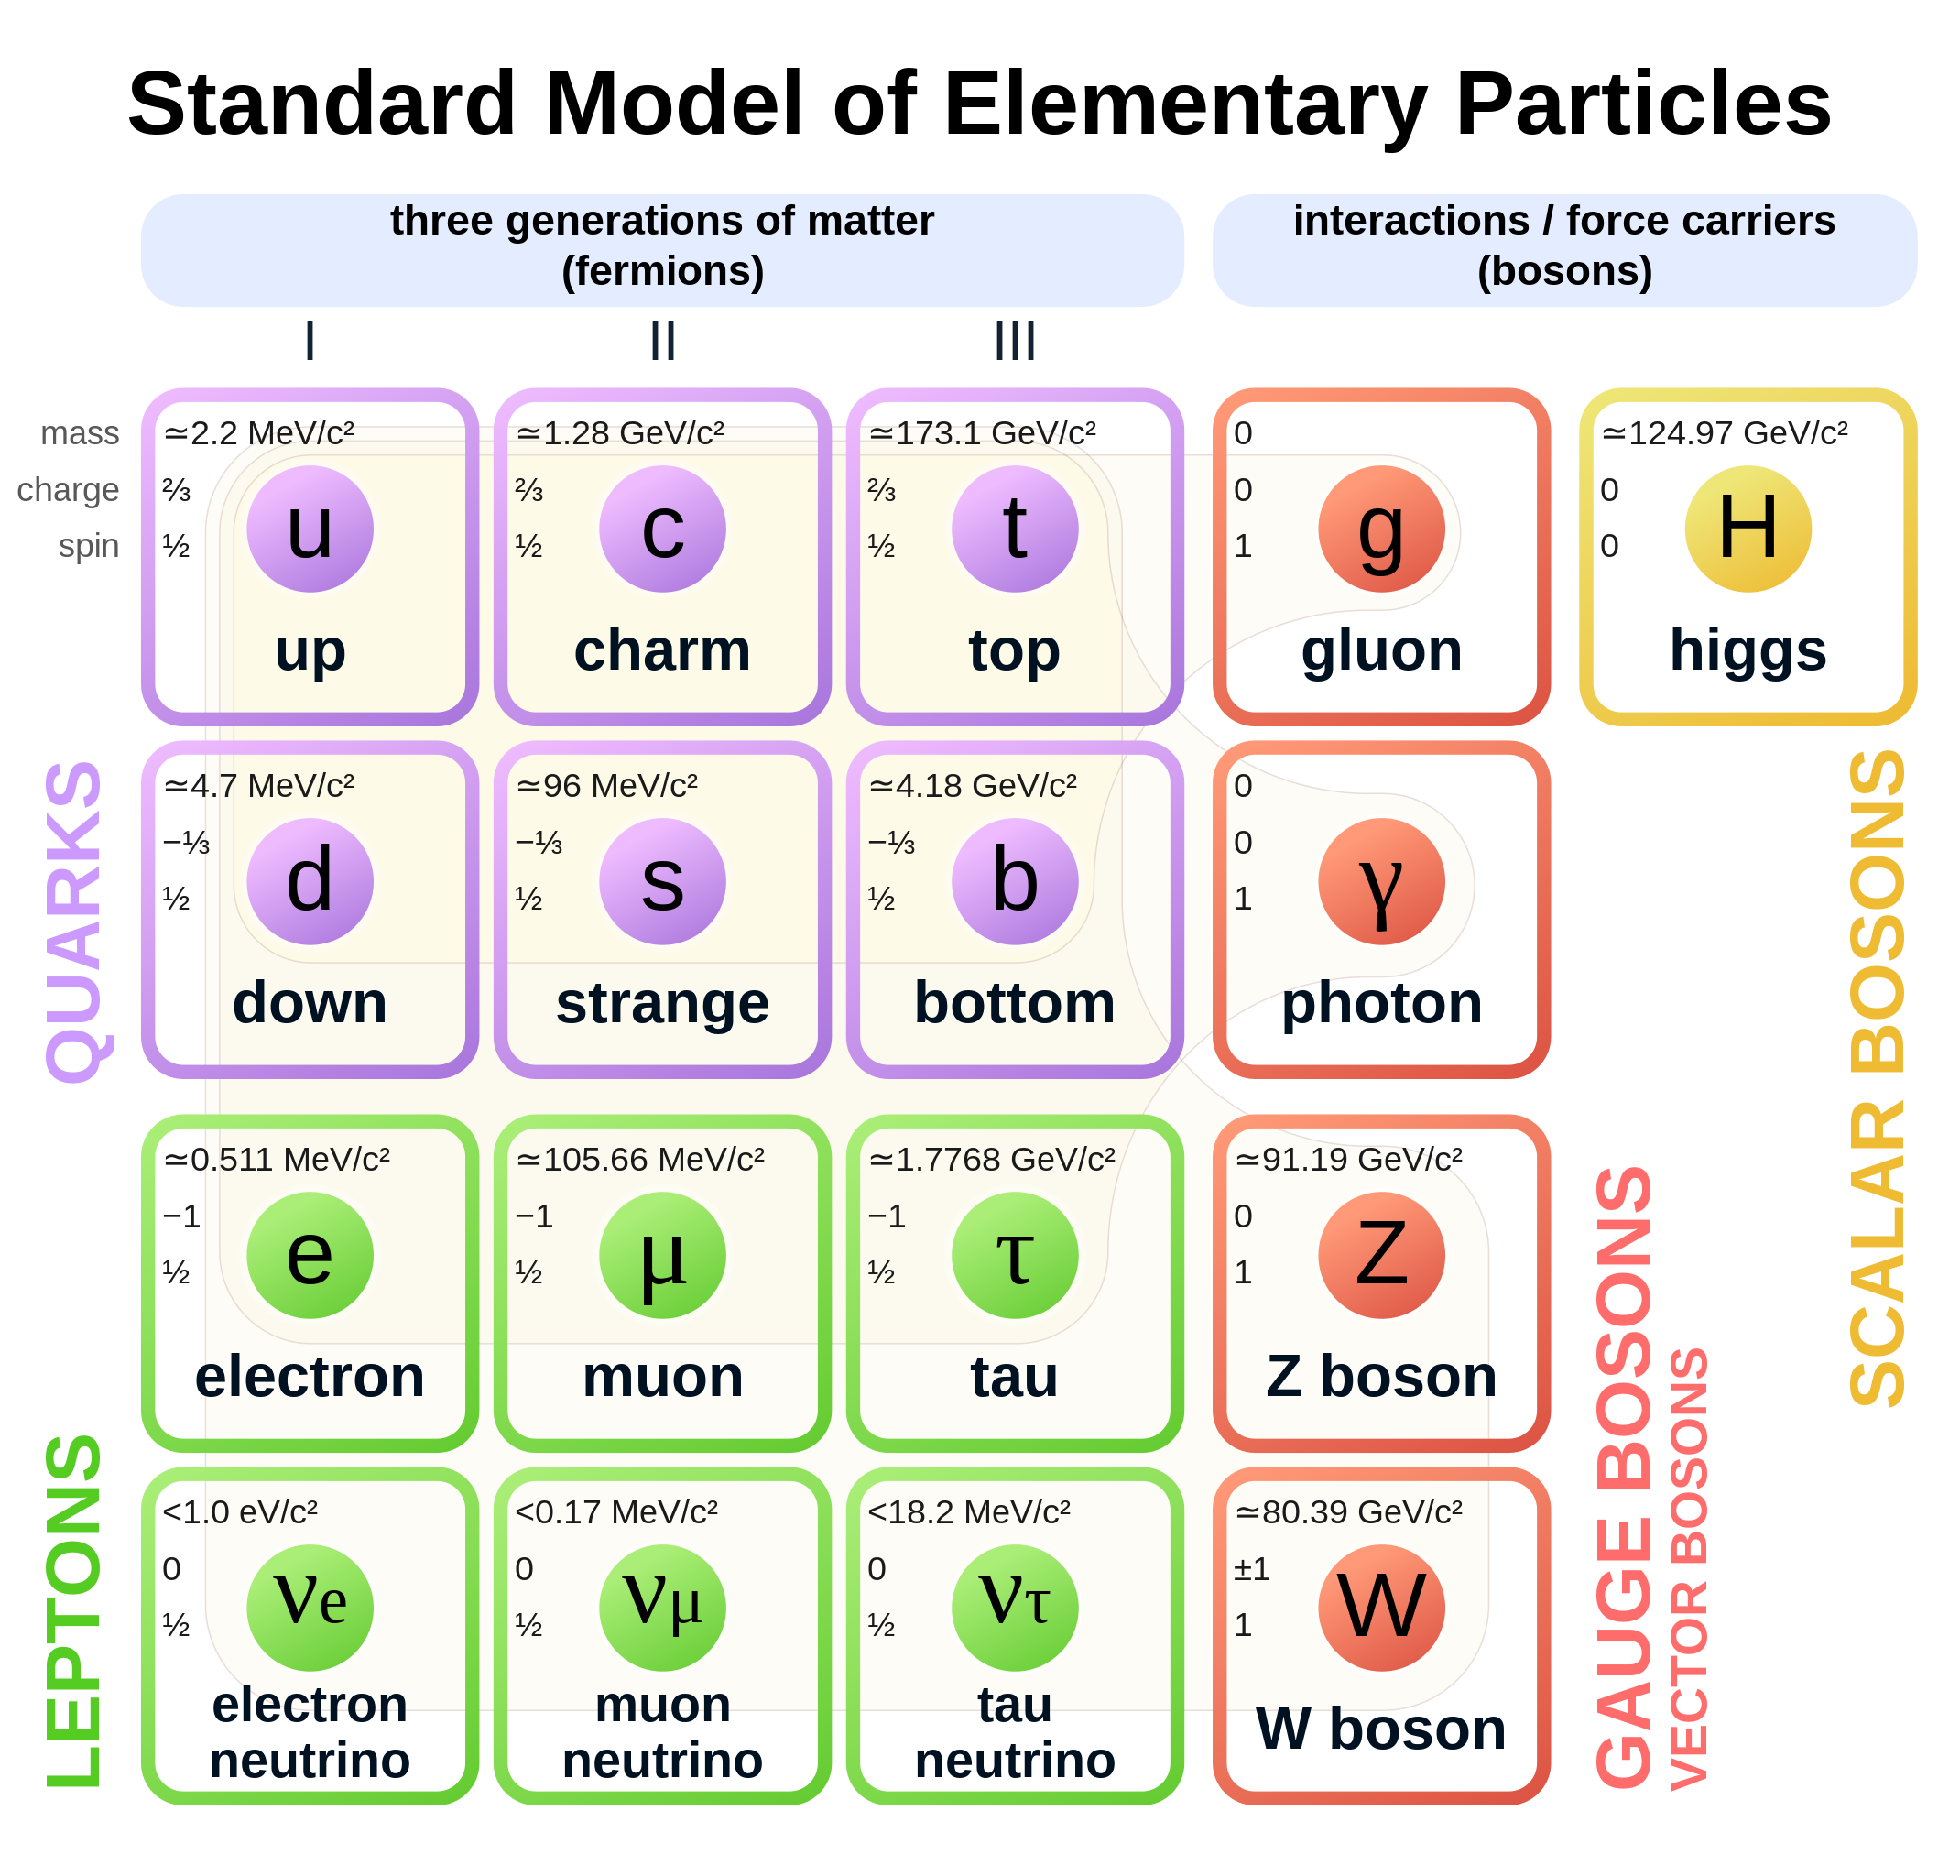
\includegraphics[scale =0.1]{figure_1/Standard_Model_of_Elementary_Particles.svg.png}
    \caption{Figure represent Standard model of particle physics. This includes three generation of quarks and leptons, along with force mediator gauge Boson, photon, and gluon. It also include the scalar Higgs bosons.}
    \label{fig:my_figure_1}
\end{figure}
\begin{itemize}
    \item \textbf{Gravity:-} The Standard Model does not consistently explain the canonical theory of gravity and the general theory of relativity from the perspective of quantum field theory, despite the fact that it corresponds to strong interaction and electroweak interaction \cite{Bilson_Thompson_2007}. The fact that quantum field theory in the field of gravity frequently collapses before reaching the Planck scale is one reason for this. As a result, we don't have a solid theory for the origins of the universe.
    
    \item \textbf{Hierarchy problem:-} The Higgs field causes spontaneous symmetry violation in the Standard Model, which introduces particle mass\cite{Higgs:1964pj}. Due to the presence of virtual particles in the Standard Model, the Higgs mass experiences substantial quantum corrections (top quarks). These adjustments are substantially larger than the Higgs real mass.\cite{Aad_2015}. 

\item \textbf{Neutrino Oscillation:-} According to the standard model, neutrinos have zero mass. But, from experiments and studies conducted in past decades have evidenced to have neutrino mass. Manually adding the neutrino mass term to the Standard Model creates a new theoretical problem\cite{neutino_1}. For example, the mass term must be very small, and it is unclear if the mass of neutrinos is generated in the Standard Model in the same way as the mass of other constituent particles\cite{Ellis_2020}.
    
    
 \item \textbf{Matter anti-Matter asymmetry:-} The universe is mainly composed of matter. However, the Standard Model predicts that if the initial conditions of the universe do not contain an imbalanced amount of matter compared to antimatter, matter and antimatter should be formed in (almost) equal amounts\cite{Dasgupta_2020}. However, the Standard Model does not have a mechanism to properly explain this asymmetry.

There are many other observed phenomena without evident explanation by the standard model, such as strong CP problem\cite{doi:10.1126/science.abk1781}, presence of Dark matter and Dark energy, and the most recent anomalous mass of the W boson-results from the CDF Collaboration\cite{CMS:2008xjf}.
\end{itemize}   



The Beyond Standard Model (BSM) needs to address phenomena that cannot be explained by the Standard Model, such as  strong CP problems, neutrino oscillations, matter-antimatter asymmetry, and the inability to explain the properties of dark matter and dark energy. \cite{https://doi.org/10.48550/arxiv.1202.1391}. Many theories have been developed to extend  SM to address some of the above issues. Some of these models are supersymmetry (SUSY)\cite{MARTIN_1998}, right-handed neutrino seesaw models \cite{neutrino_mass_model}, vector-like quarks, and extra-dimensional prediction models. Vector like Quark (VLQ) model predicts the presence of giant particles, Non-chiral quark. Proton-proton(pp) collisions can form these quarks at 13 TeV at the LHC. VLQ is the primary focus of this analysis and will be discussed in detail in the following sections.



%  Surprisingly, all these extensions of  SM predict new particles. The SUSY model predicts the presence of  supersymmetric partners for all SM particles with different spin  units. This means that all fermions have supersymmetric boson partners and vice versa. 
%  The seesaw model introduces a sterile heavy right-handed neutrino to explain this much. 
%  A small left-handed neutrino mass that appears in  SM. The additional dimensions predict the existence of some new dimensions in addition to the usual four space-time dimensions. These may explain why gravity is so much weaker than  other fundamental forces of nature. According to these theories, gravitons (carriers of gravitational force) can penetrate these additional dimensions, but other SM particles cannot. Vectorlike Quark (VLQ) model predicts the presence of giant particles  Non-chiral quark. These quarks can be formed by proton-proton (pp) collisions at 13 TeV at the LHC. VLQ is the subject of this research and will be discussed in detail in the next section.

\section{Vector-like Quarks(VLQ)}

Standard model(SM) is consists of only chiral fermions, where the left-handed and right-handed fermionic fields are conserved, which transform differently under the SU(2) gauge transformations. As a result, the Dirac mass term m becomes $\psi\Bar{\psi}$\cite{Aguilar_Arevalo_2018}. SM with charged fermions gain mass via the (BroutEnglertHiggs) BEH mechanism\cite{PhysRevLett.13.321}\cite{Higgs:1964pj}. In particular,  W bosons only interact with SM left-handed fermions. 

However, some theoretical models predict the existence of new heavy quarks that are not Chiral
in nature. Such models include compound Higgs\cite{10.3389/fphy.2019.00022}, Randall Sundrum
models\cite{Randall_1999}, and Grand Unified Theory (GUT)\cite{Kang_2008} and Little Higgs
model\cite{Arkani_Hamed_2002}. Unlike SM quarks, these quarks are Vector coupled to the charged current. These quarks are heavier partners for top and bottom quarks\cite{Angelescu_2016}. That is, a $T'$ quark with a charge of $ \frac{2}{3} $ e and a $B'$ quark with a charge of $ -\frac{1}{3} $ e. These predicted models help to cancel the divergent quantum loop correction introduced by the top quark into the Higgs mass. These new quarks can interact with SM particles and  decay to one-third generation quarks and  heavy bosons. For such non-chiral fermions, the Dirac mass term m $ \psi\Bar{\psi} $ is not prohibited. The only way to determine the mass of these particles is to find them experimentally.  Previous searches for these VLQs were performed by both ATLAS and CMS at the center of mass energy ($ \sqrt{s}$) = 7, 8, and 13TeV \cite{Aad_2014}. It is a colored spin 1/2 fermion \cite{VLQ_1}. 
% The left-handed and right-handed components are transformed in the standard model gauge group as well. Therefore different SM chiral quarks, their masses are not produced by the Yukawa interaction with the Higgs. 
%  It is a  boson and has little effect on the cross-section of the Higgs boson. Various modifications 
%  The new physics els introduces vector-like quarks. 
%  Such models include composite Higgs models \cite{neutrino_mass_model}, Little-Higgs model \cite{Perelstein_2004} \cite{Matsedonskyi_2013},  Extradimension model [\cite{Randall_1999}, etc. 
%  This paper investigates the specific separation of the Tprime ($T`$) quark decay topology  described in the next section.
 
 
 







The vector-like top quark partner $T'$ has two generation modes, as shown in \autoref{fig:threeVLQgraphs}\cite{Belyaev_2021}. One is due to
pair production where  there is a strong interaction(\autoref{fig:threesinx}) and the other is a single production mode
with electroweak interactions(\autoref{fig:yequalsx}). The VLQ pairs to SM quarks q and weak bosons V$\in$ \{W, Z, H \},
via QqV vertices, as shown in \autoref{fig:threeVLQgraphs} and in \autoref{eq:label_1222}

\begin{equation*}\label{eq:label_1222}
\begin{split}
 T' \longrightarrow tW, T' \longrightarrow tZ, T' \longrightarrow tH  \\
   B' \longrightarrow bW, B' \longrightarrow bZ, B' \longrightarrow bH
\end{split}
\end{equation*}


\begin{figure}[H]
     \centering
     \begin{subfigure}[b]{0.47\textwidth}
         \centering
         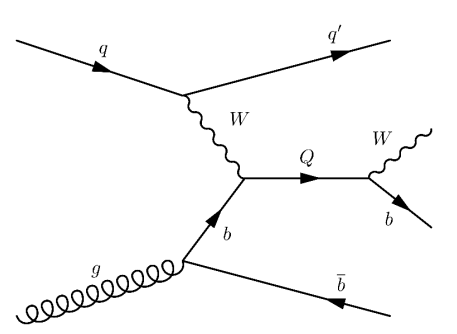
\includegraphics[width=\textwidth]{figure_1/1.png}
         \caption{Single production of VLQ, $T'$.}
         \label{fig:yequalsx}
     \end{subfigure}
     \hfill
     \begin{subfigure}[b]{0.47\textwidth}
         \centering
         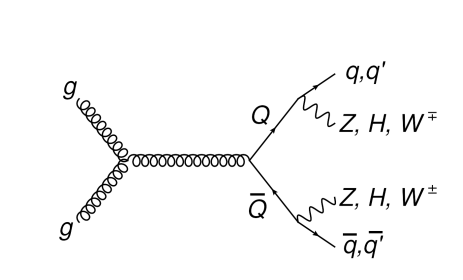
\includegraphics[width=\textwidth]{figure_1/2.png}
         \caption{Double production of VLQ, $T'$.}
         \label{fig:threesinx}
     \end{subfigure}
     \hfill
    %  \begin{subfigure}[b]{0.3\textwidth}
    %      \centering
    %      \includegraphics[width=\textwidth]{graph3}
    %      \caption{$y=5/x$}
    %      \label{fig:five over x}
    %  \end{subfigure}
        \caption{The different mode of generation modes of the vector-like quark, $T'$.}
        \label{fig:threeVLQgraphs}
\end{figure}





The $T'$ quark combined with tW, tZ, or tH into the corresponding $T'$ quark. 
 In this thesis, the study  has been considered with a single VLQ, top quark partner $T'$  generated in a proton-proton (pp) collision at the center of mass energy ($\sqrt{s}$) = 13TeV, with processes pp $\longrightarrow$ $T'$ at LHC(discussed in \autoref{CMS}). The focus is on electroweak generation, $T'$ qH channel from the Higgs boson to two photons (H $\longrightarrow\gamma\gamma$) and is generated by the Higgs boson decay $T'$ $\longrightarrow$ tH. The leading order (LO) Feynman diagram for the $T'$ is shown in \autoref{fig:my_label_Feynman}. This analysis is designed to be sensitive to  top quark lepton decay and Higgs boson decaying into two photons. The experimental features are the resonance peak of the invariant mass spectrum of the two photons and another resonance peak of the invariant tH  mass spectrum. A detailed description of $T'$ and the corresponding backgrounds can be seen in \autoref{signal_background}. 
The separation of signal, for the $T'$ quark from the large backgrounds processes have been helped with the use Deep neural network(DNN) which have been discussed briefly in next section.


   




\begin{figure}[H]
    \centering
    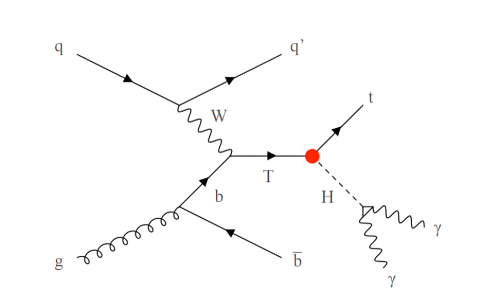
\includegraphics{figure_4/3.png}
    \caption{Feynman diagram for single vector-like quark(VLQ), ${T'}$ production. $T'$ is produced with the electroweak interaction of W boson and b quark. As being a resonance particle, $T'$ decay in moment into Higgs boson(H) and standard model top quark(t). Higgs(H) further goes on giving diphoton($\gamma\gamma$, while top quark decays to b quark and W boson. W boson decays leptonically to electron(e) and electron neutrino($\nu_e$).}
    \label{fig:my_label_Feynman}
\end{figure}

\section{Deep Neural Network(DNN)}
Neural networks, also known as artificial neural networks(ANN), are structures inspired by the human brain and also mimic the connectivity of biological signals to one another, as in \autoref{fig:my_label_NN_ANNN}.
In the neural network, node takes the input as a real number (the weighted sum of the connected outputs from the previous layer) and performs a non-linear transformation to form that output\cite{Bourilkov_2019}.
These non-linear transformation functions are known as the activation function. A typical activation function is: Sigmoid (logistics) and Tanh (output is limited to the following for all input values), and the normalized linear unit ReLU(max(0, x)) or the positive part of the argument. Each neural network consists of at least an input, an output, and one or more hidden layers\cite{Sarker2021}. This is part of Deep learning. We represent deep NN as DNN. The learning can be supervised depending on pairs of inputs with known outputs for training, or unsupervised, or semi-supervised. A cost or loss function measures the “distance” between the current and the desired outcomes, where our main goal is to make a model loss as little as possible to train the model. Traditional optimization aims to minimize the cost function of available (training) data. The main goal of ML is to generalize or minimize the cost of hidden or test data. At each step,  backpropagation based on the differential chain rule can adjust the weights of all edges to reduce the cost function slightly. This is Stochastic Gradient Descent (SGD), which further in detailed discussed in \autoref{ML}. 
Aside from being universal approximators (i.e., they estimate probability densities or posterior probabilities to arbitrary precision), neural networks are an extremely useful tool due to the short computational time required in their training ( in a majority of applications in HEP)\cite{https://doi.org/10.48550/arxiv.2003.05199}. The DNN has been used for the signal and background separation, which have discussed briefly in next section and in detailed \autoref{signal_background}.
\begin{figure}[h]
    \centering
    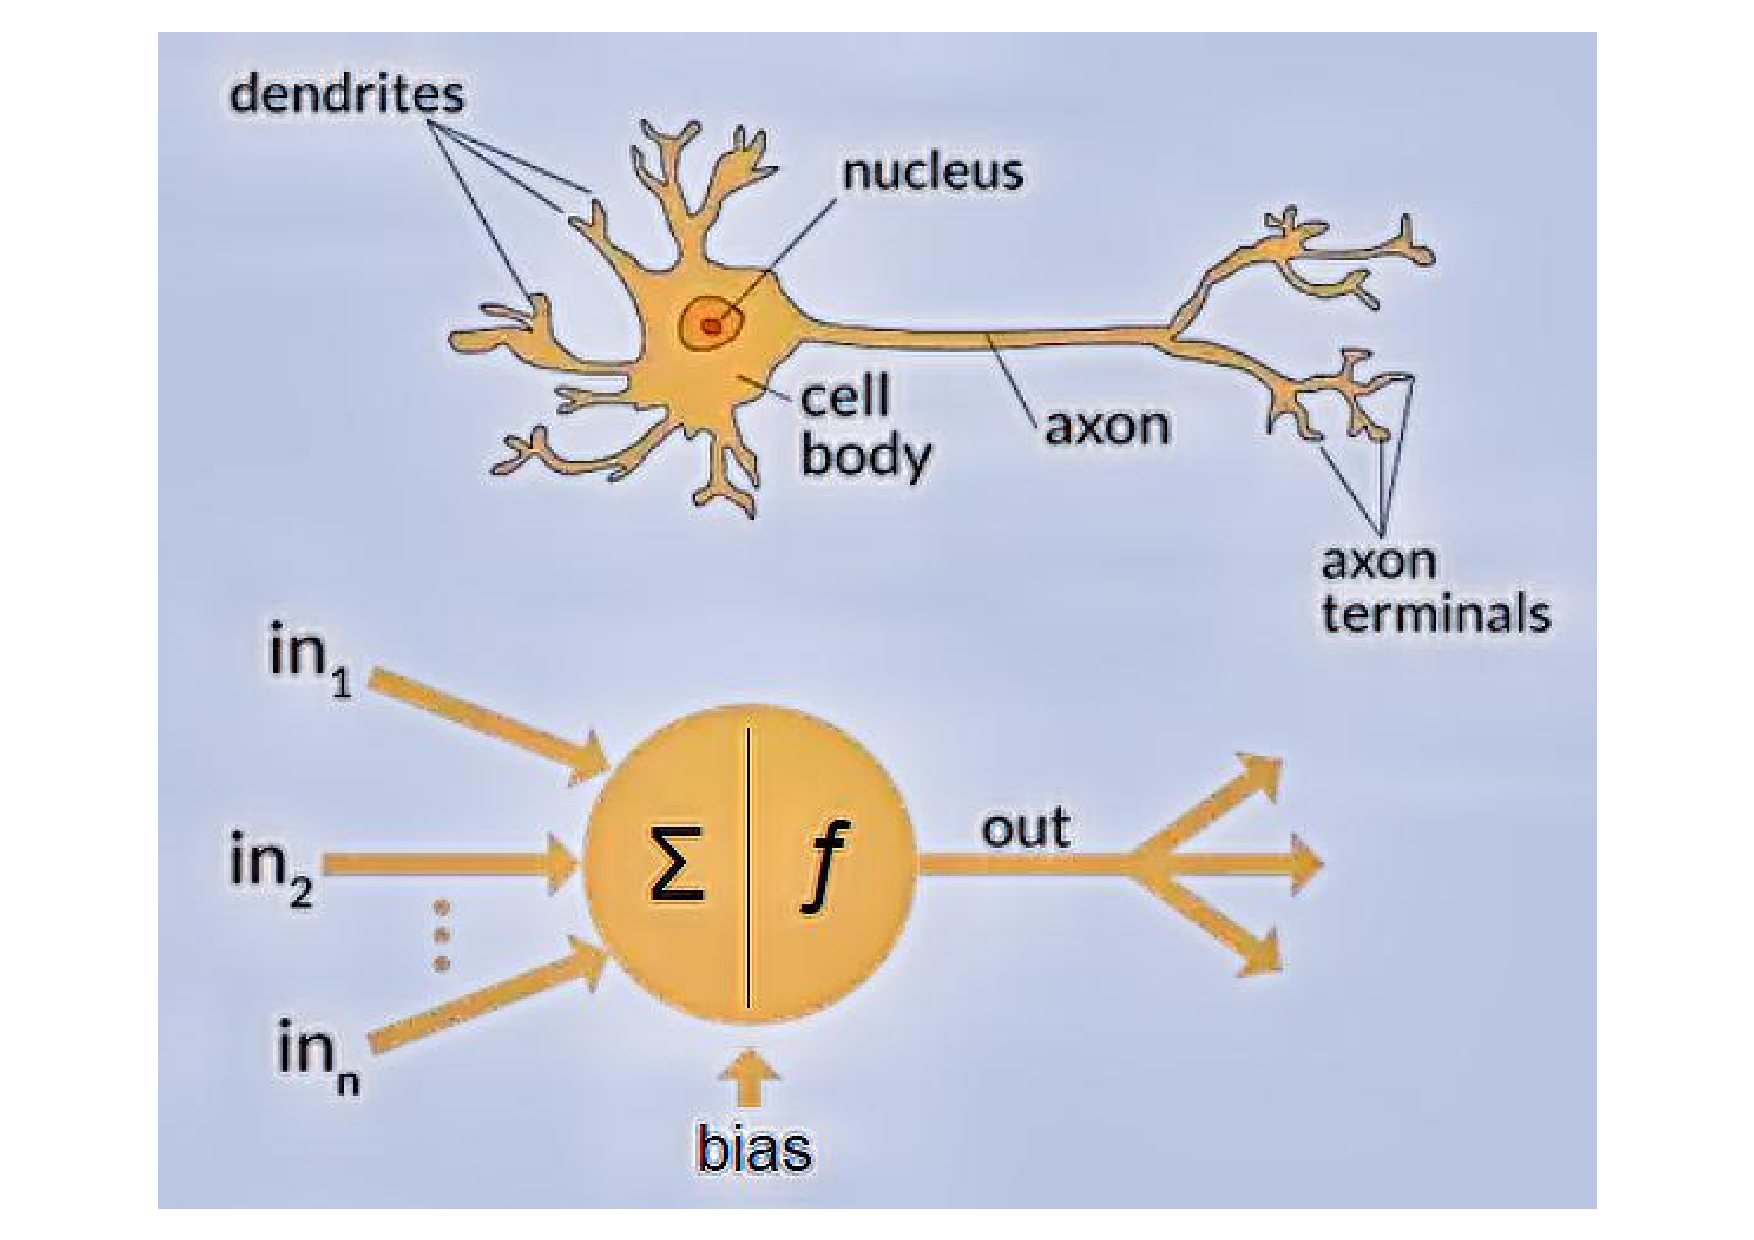
\includegraphics[scale=0.4]{Figure/img_neuron.pdf}
    \caption{A biological and an artificial neuron}
    \label{fig:my_label_NN_ANNN}
\end{figure}

\section{Signal and Background}

The Deep Neural network(DNN) has been trained with the Tprime($T'$) at different mass point from [600,1200]GeV as signal and standard
model higgs(SMH) as the backgrounds which also decays to the leptons. The different SMH backgrounds used in training are
ttH($\longrightarrow$ $\gamma \gamma$), tH($\longrightarrow$ $\gamma \gamma$)q, VBFH($\longrightarrow$ $\gamma \gamma$),
VH($\longrightarrow$ $\gamma \gamma$), and ggH(H($\longrightarrow$ $\gamma \gamma$). All of samples(signal and background) have the
similar final state topology with H $\longrightarrow$ $\gamma \gamma$.

The DNN training model output tested over the Non-Resonant background(tt$\gamma \gamma$, ttJets, tgJets, gJets, and DiphotonJets), which plotted as ratio plot after normalizing with the data and the monte carlo, which have been further discussed in details in \autoref{signal_background}. 


%%%Objective of the experiment%%%% 
The analysis strategy adopted in this thesis with the discussion of the combined tools used for the statistical limit calculation on each mass points of the $T'$ from [600, 1200] GeV are discussed in \autoref{AN}. The DNN model have been compared with the existing analysis using another multivariate techniques, Boosted Decision Tree(BDT) and the output results can be seen in the \autoref{R_D}. The expected limit at 95\% confidence intervals(CLs) on $T'$ production processes have been extracted at each $T'$ mass in the range [600,1200] using the DNN based selection criteria, as well as for the present CMS analysis(BDT).
















    







% \url{https://lhc-machine-outreach.web.cern.ch/lhc_in_pictures.htm}
% \url{https://lhc-closer.es/taking_a_closer_look_at_lhc/1.standard_model}


% \noindent\fbox{%
%     \parbox{\textwidth}{%
% 1.   Dawson, S. et al. Higgs Working Group Report of the
% Snowmass 2013 Community Planning Study, Preprint at
% http://arxiv.org/abs/1310.8361 (2013).
% https://home.cern/science/physics/matter-antimatter-asymmetry-problem
% 2. Neyman, J. & Pearson, E. Philosophical Transactions of
% the Royal Society 231, 694–706 (1933).
% 3.  Womersley, J. (February 2005). "Beyond the Standard Model" (PDF). Symmetry Magazine. Archived from the original (PDF) on 2007-10-17. Retrieved 2010-11-23.
% 4. S. P. Martin, Adv. Ser. Direct. High Energy Phys.21 (2010), 1-153, arXiv:hep-ph/9709356.
% 5 S.F. King, Rept.Prog.Phys. 67 (2004) 107-158, arXiv:hep-ph/0310204
% 6 M. Shifman, Int.J.Mod.Phys.A25:199-225, 2010, arXiv:0907.3074.
% R. Contino, L. Da Rold, and A. Pomarol, “Light custodians in natural composite Higgs
% models”, Physical Review D 75 (March, 2007) 055014,
% doi:10.1103/PhysRevD.75.055014. arXiv: hep-ph/0612048.
% [6] R. Contino, T. Kramer, M. Son, and R. Sundrum, “Warped/Composite Phenomenology
% Simplified”, Journal of High Energy Physics 2007 (May, 2007) 074–074,
% doi:10.1088/1126-6708/2007/05/074. arXiv: hep-ph/0612180.
% [7] D. B. Kaplan, “Flavor at ssc energies: A new mechanism for dynamically generated
% fermion masses”, Nuclear Physics B 365 (November, 1991) 259–278,
% doi:10.1016/S0550-3213(05)80021-5.
% [8] M. J. Dugan, H. Georgi, and D. B. Kaplan, “Anatomy of a composite Higgs model”,
% Nuclear Physics B 254 (January, 1985) 299–326,
% doi:10.1016/0550-3213(85)90221-4.
% [9] S. Blasi and F. Goertz, “Softened Goldstone-Symmetry Breaking”, Physical Review Letters
% 123 (November, 2019) 221801, doi:10.1103/PhysRevLett.123.221801. arXiv:
% 1903.06146.
% [10] M. Perelstein, M. E. Peskin, and A. Pierce, “Top Quarks and Electroweak Symmetry
% Breaking in Little Higgs Models”, Physical Review D 69 (April, 2004) 075002,
% doi:10.1103/PhysRevD.69.075002. arXiv: hep-ph/0310039.
% [11] O. Matsedonskyi, G. Panico, and A. Wulzer, “Light Top Partners for a Light Composite
% Higgs”, Journal of High Energy Physics 2013 (January, 2013) 164,
% doi:10.1007/JHEP01(2013)164. arXiv: 1204.6333.
% [12] M. Schmaltz and D. Tucker-Smith, “Little Higgs Review”, Annual Review of Nuclear and
% Particle Science 55 (December, 2005) 229–270,
% doi:10.1146/annurev.nucl.55.090704.151502. arXiv: hep-ph/0502182.
% [13] L. Randall and R. Sundrum, “A Large Mass Hierarchy from a Small Extra Dimension”,
% Physical Review Letters 83 (October, 1999) 3370–3373,
% doi:10.1103/PhysRevLett.83.3370. arXiv: hep-ph/9905221.
%     }%
% }